










%%-------------------------------------------------------------------------------%%
%% Give full data tables for both analyses.
%%-------------------------------------------------------------------------------%%










\begin{landscape}

% latex table generated in R 3.2.4 by xtable 1.8-2 package
% Sun Apr 17 12:14:27 2016
\begingroup\tiny
\begin{longtable}{@{}llrrrrrrrrrl@{}}
\caption[
Raw data for both analyses.
]{
Raw data for both analyses.
Range Length is the distance between furthest apart points in the species range.
Dmax is the distance between furthest apart $F_{ST}$ sampling locations.
The references are for the $F_{ST}$ data only.
} \\ 
  \toprule
Family & Binomial & Virus Sp. & Subsp. & Gene Flow & Mass & Range Size & Scholar & PubMed & Range Length & Dmax & Reference \\ 
  &  &  &  &  & (g) & ($\times 10^{9}$km$^2$) &  &  & (km) & (km) &  \\ 
   \midrule
\endfirsthead 
\caption[]{
Raw data for both analyses.
Range Length is the distance between furthest apart points in the species range.
Dmax is the distance between furthest apart $F_{ST}$ sampling locations.
The references are for the $F_{ST}$ data only.
}\\
\toprule
Family & Binomial & Virus Sp. & Subsp. & Gene Flow & Mass & Range Size & Scholar & PubMed & Range Length & Dmax & Reference \\
   &  &  &  &  & (g) & ($\times 10^{9}$km$^2$) &  &  & (km) & (km) &  \\
 \midrule 
\endhead 
Megadermatidae & \emph{Macroderma gigas} & 0 &  & 0.25 & 124.37 & 1078.95 & 769 & 13 & 3609.23 & 3148 & \cite{wilmer1999genetic} \\ 
  Miniopteridae & \emph{Miniopterus natalensis} & 0 &  & 0.08 & 10.43 & 3784.83 & 180 & 5 & 6657.28 & 1706 & \cite{miller2003strong} \\ 
  Miniopteridae & \emph{Miniopterus schreibersii} & 12 &  & 1.86 & 11.46 & 3707.97 & 3090 & 64 & 7050.77 & 2649 & \cite{witsenburg2015haemosporidian} \\ 
  Phyllostomidae & \emph{Macrotus waterhousii} & 0 &  & 2.33 & 16.27 & 802.74 & 594 & 15 & 4298.38 & 935 & \cite{burns2014correlates} \\ 
  Pteropodidae & \emph{Rousettus obliviosus} & 0 &  & 13.76 & 45.32 & 1.67 & 52 & 0 & 174.92 & 160 & \cite{goodman2010phylogeny} \\ 
  Pteropodidae & \emph{Thoopterus nigrescens} & 0 &  & 0.14 & 66.12 & 182.87 & 52 & 0 & 1388.27 & 620 & \cite{burns2014correlates} \\ 
  Vespertilionidae & \emph{Myotis ciliolabrum} & 0 &  & 12.38 & 4.89 & 1388.27 & 592 & 5 & 2150.93 & 473 & \cite{burns2014correlates} \\ 
  Vespertilionidae & \emph{Myotis macropus} & 0 &  & 0.44 & 9.8 & 1326.85 & 214 & 0 & 3644.70 & 883 & \cite{burns2014correlates} \\ 
  Hipposideridae & \emph{Hipposideros speoris} & 2 & 1 & 0.07 & 10.39 & 1225.28 & 603 & 9 & 2801.74 & 1175 & \cite{chinnasamy2013genetic} \\ 
  Phyllostomidae & \emph{Desmodus rotundus} & 7 & 1 & 1.29 & 33.16 & 17726.52 & 6810 & 265 & 9314.10 & 2252 & \cite{burns2014correlates} \\ 
  Phyllostomidae & \emph{Macrotus californicus} & 1 & 1 & 1.26 & 11.83 & 643.20 & 808 & 15 & 2139.83 & 590 & \cite{burns2014correlates} \\ 
  Pteropodidae & \emph{Cynopterus sphinx} & 3 & 6 & 5.08 & 44.71 & 6456.51 & 1620 & 53 & 6821.48 & 3915 & \cite{burns2014correlates} \\ 
  Pteropodidae & \emph{Pteropus alecto} & 6 & 4 & 5.31 & 610.13 & 1354.21 & 1530 & 49 & 5064.99 & 2961 & \cite{webb1996mobility} \\ 
  Pteropodidae & \emph{Pteropus conspicillatus} & 2 & 2 & 2.92 & 760.71 & 219.53 & 465 & 15 & 3294.68 & 993 & \cite{fox2006population} \\ 
  Pteropodidae & \emph{Pteropus poliocephalus} & 3 & 1 & 8.80 & 702.78 & 249.32 & 1950 & 54 & 1844.19 & 721 & \cite{webb1996mobility} \\ 
  Pteropodidae & \emph{Pteropus scapulatus} & 7 & 1 & 4.34 & 380.35 & 3038.11 & 707 & 19 & 4053.21 & 2625 & \cite{burns2014correlates} \\ 
  Pteropodidae & \emph{Rousettus leschenaultii} & 11 & 3 & 17.73 & 84.88 & 6764.79 & 848 & 0 & 6795.10 & 3828 & \cite{burns2014correlates} \\ 
  Pteropodidae & \emph{Rousettus madagascariensis} & 1 & 1 & 31.12 & 65.72 & 292.74 & 135 & 2 & 1483.04 & 1366 & \cite{burns2014correlates} \\ 
  Rhinolophidae & \emph{Rhinolophus ferrumequinum} & 9 & 7 & 2.78 & 22.59 & 9747.14 & 5070 & 85 & 12178.06 & 9670 & \cite{burns2014correlates} \\ 
  Vespertilionidae & \emph{Lasiurus borealis} & 1 & 1 & 19.61 & 12.33 & 4881.50 & 3460 & 28 & 4185.94 & 2198 & \cite{vonhofgenetic} \\ 
  Vespertilionidae & \emph{Myotis lucifugus} & 8 & 5 & 7.64 & 7.8 & 12040.88 & 9720 & 298 & 6671.21 & 5173 & \cite{vonhof2015range} \\ 
  Vespertilionidae & \emph{Myotis myotis} & 6 & 2 & 3.45 & 25.59 & 3874.58 & 8880 & 137 & 4377.75 & 2786 & \cite{burns2014correlates} \\ 
  Vespertilionidae & \emph{Myotis ricketti} & 3 & 1 & 2.38 & 22.5 & 987.18 & 421 & 11 & 2741.15 & 2272.57 & \cite{lu2013phylogeography} \\ 
  Vespertilionidae & \emph{Nyctalus noctula} & 8 & 4 & 20.71 & 28.48 & 8033.97 & 4670 & 37 & 10238.26 & 4015 & \cite{burns2014correlates} \\ 
  Emballonuridae & \emph{Rhynchonycteris naso} & 1 & 1 &  & 4.14 & 11508.83 & 607 & 2 &  &  &  \\ 
  Emballonuridae & \emph{Saccolaimus flaviventris} & 1 & 1 &  & 45.25 & 6053.68 & 342 & 3 &  &  &  \\ 
  Emballonuridae & \emph{Taphozous melanopogon} & 4 & 5 &  & 25.99 & 5624.37 & 503 & 15 &  &  &  \\ 
  Emballonuridae & \emph{Taphozous perforatus} & 2 & 4 &  & 24.43 & 2114.92 & 264 & 5 &  &  &  \\ 
  Hipposideridae & \emph{Aselliscus stoliczkanus} & 1 & 1 &  & 6.09 & 1362.32 & 128 & 9 &  &  &  \\ 
  Hipposideridae & \emph{Hipposideros armiger} & 5 & 4 &  & 49.99 & 4475.41 & 656 & 26 &  &  &  \\ 
  Hipposideridae & \emph{Hipposideros bicolor} & 1 & 7 &  & 8.39 & 1584.43 & 371 & 4 &  &  &  \\ 
  Hipposideridae & \emph{Hipposideros caffer} & 3 & 4 &  & 9.46 & 6348.39 & 458 & 6 &  &  &  \\ 
  Hipposideridae & \emph{Hipposideros cineraceus} & 1 & 2 &  & 3.84 & 2203.63 & 164 & 0 &  &  &  \\ 
  Hipposideridae & \emph{Hipposideros commersoni} & 1 & 1 &  & 89.99 & 513.16 & 429 & 0 &  &  &  \\ 
  Hipposideridae & \emph{Hipposideros diadema} & 2 & 15 &  & 46.9 & 3318.84 & 472 & 4 &  &  &  \\ 
  Hipposideridae & \emph{Hipposideros lankadiva} & 1 & 1 &  & 44.76 & 712.59 & 188 & 2 &  &  &  \\ 
  Hipposideridae & \emph{Hipposideros larvatus} & 2 & 5 &  & 19.95 & 3287.88 & 398 & 7 &  &  &  \\ 
  Hipposideridae & \emph{Hipposideros pomona} & 2 & 3 &  & 6.2 & 2840.90 & 226 & 5 &  &  &  \\ 
  Megadermatidae & \emph{Megaderma lyra} & 2 & 2 &  & 39.27 & 6042.09 & 1370 & 32 &  &  &  \\ 
  Molossidae & \emph{Chaerephon plicatus} & 2 & 5 &  & 21.83 & 2462.34 & 62 & 0 &  &  &  \\ 
  Molossidae & \emph{Chaerephon pumilus} & 4 & 1 &  & 10.98 & 7240.27 & 177 & 0 &  &  &  \\ 
  Molossidae & \emph{Cynomops abrasus} & 1 & 4 &  & 35.39 & 10671.17 & 143 & 2 &  &  &  \\ 
  Molossidae & \emph{Cynomops planirostris} & 1 & 1 &  & 12.84 & 11450.26 & 138 & 0 &  &  &  \\ 
  Molossidae & \emph{Eumops auripendulus} & 1 & 2 &  & 28.49 & 14106.77 & 343 & 2 &  &  &  \\ 
  Molossidae & \emph{Eumops glaucinus} & 1 & 2 &  & 36.2 & 11385.12 & 545 & 5 &  &  &  \\ 
  Molossidae & \emph{Eumops perotis} & 1 & 3 &  & 50.97 & 11695.63 & 859 & 5 &  &  &  \\ 
  Molossidae & \emph{Molossops neglectus} & 1 & 1 &  & 11 & 6515.61 & 166 & 0 &  &  &  \\ 
  Molossidae & \emph{Molossus molossus} & 7 & 7 &  & 13.7 & 15767.72 & 2220 & 68 &  &  &  \\ 
  Molossidae & \emph{Molossus rufus} & 9 & 1 &  & 120 & 14800.28 & 629 & 11 &  &  &  \\ 
  Molossidae & \emph{Mops condylurus} & 3 & 4 &  & 26.59 & 9123.92 & 310 & 5 &  &  &  \\ 
  Molossidae & \emph{Nyctinomops laticaudatus} & 1 & 5 &  & 13.12 & 13101.23 & 511 & 11 &  &  &  \\ 
  Molossidae & \emph{Nyctinomops macrotis} & 1 & 1 &  & 16.38 & 15743.81 & 641 & 8 &  &  &  \\ 
  Molossidae & \emph{Tadarida brasiliensis} & 5 & 9 &  & 12.61 & 13833.40 & 5400 & 131 &  &  &  \\ 
  Molossidae & \emph{Tadarida teniotis} & 1 & 2 &  & 28.07 & 3743.23 & 1160 & 7 &  &  &  \\ 
  Mormoopidae & \emph{Mormoops megalophylla} & 3 & 4 &  & 16.09 & 3738.69 & 806 & 9 &  &  &  \\ 
  Mormoopidae & \emph{Pteronotus davyi} & 5 & 3 &  & 9.52 & 3471.86 & 680 & 2 &  &  &  \\ 
  Mormoopidae & \emph{Pteronotus parnellii} & 7 & 9 &  & 19.59 & 8592.98 & 2400 & 128 &  &  &  \\ 
  Natalidae & \emph{Natalus stramineus} & 1 & 6 &  & 5.68 & 4.47 & 675 & 4 &  &  &  \\ 
  Natalidae & \emph{Natalus tumidirostris} & 4 & 3 &  & 6.3 & 1593.55 & 19 & 0 &  &  &  \\ 
  Nycteridae & \emph{Nycteris gambiensis} & 3 & 1 &  & 7.13 & 1860.95 & 62 & 0 &  &  &  \\ 
  Nycteridae & \emph{Nycteris nana} & 1 & 1 &  & 6.98 & 2938.13 & 42 & 0 &  &  &  \\ 
  Nycteridae & \emph{Nycteris thebaica} & 1 & 8 &  & 9.2 & 14397.36 & 625 & 7 &  &  &  \\ 
  Phyllostomidae & \emph{Anoura caudifer} & 1 & 1 &  & 10.81 & 8856.50 & 177 & 0 &  &  &  \\ 
  Phyllostomidae & \emph{Anoura geoffroyi} & 9 & 3 &  & 15.15 & 7791.08 & 1140 & 11 &  &  &  \\ 
  Phyllostomidae & \emph{Artibeus cinereus} & 3 & 1 &  & 12.7 & 3466.55 & 463 & 3 &  &  &  \\ 
  Phyllostomidae & \emph{Artibeus fimbriatus} & 1 & 1 &  & 63.89 & 1480.43 & 477 & 4 &  &  &  \\ 
  Phyllostomidae & \emph{Artibeus jamaicensis} & 12 & 13 &  & 43.63 & 1932.23 & 3950 & 68 &  &  &  \\ 
  Phyllostomidae & \emph{Artibeus lituratus} & 13 & 3 &  & 59.3 & 14235.95 & 2800 & 64 &  &  &  \\ 
  Phyllostomidae & \emph{Artibeus phaeotis} & 5 & 4 &  & 11.69 & 3737.37 & 354 & 0 &  &  &  \\ 
  Phyllostomidae & \emph{Carollia brevicauda} & 2 & 1 &  & 14.85 & 10749.19 & 22 & 0 &  &  &  \\ 
  Phyllostomidae & \emph{Carollia perspicillata} & 15 & 1 &  & 19.23 & 13796.36 & 4040 & 126 &  &  &  \\ 
  Phyllostomidae & \emph{Carollia subrufa} & 2 & 1 &  & 15.84 & 212.26 & 230 & 0 &  &  &  \\ 
  Phyllostomidae & \emph{Chrotopterus auritus} & 1 & 1 &  & 78.26 & 13116.79 & 955 & 4 &  &  &  \\ 
  Phyllostomidae & \emph{Diaemus youngi} & 1 & 1 &  & 36.71 & 13059.18 & 725 & 11 &  &  &  \\ 
  Phyllostomidae & \emph{Diphylla ecaudata} & 1 & 1 &  & 28.11 & 8092.44 & 1010 & 13 &  &  &  \\ 
  Phyllostomidae & \emph{Glossophaga commissarisi} & 1 & 3 &  & 9.15 & 3716.73 & 406 & 7 &  &  &  \\ 
  Phyllostomidae & \emph{Glossophaga morenoi} & 1 & 3 &  & 8.54 & 327.07 & 146 & 0 &  &  &  \\ 
  Phyllostomidae & \emph{Glossophaga soricina} & 8 & 5 &  & 9.97 & 14858.41 & 3460 & 90 &  &  &  \\ 
  Phyllostomidae & \emph{Leptonycteris curasoae} & 1 & 1 &  & 25.27 & 840.36 & 1280 & 19 &  &  &  \\ 
  Phyllostomidae & \emph{Leptonycteris nivalis} & 1 & 1 &  & 24.26 & 949.99 & 678 & 5 &  &  &  \\ 
  Phyllostomidae & \emph{Lonchophylla robusta} & 1 & 1 &  & 13.72 & 1116.13 & 248 & 0 &  &  &  \\ 
  Phyllostomidae & \emph{Lonchophylla thomasi} & 1 & 1 &  & 7.09 & 8383.35 & 282 & 0 &  &  &  \\ 
  Phyllostomidae & \emph{Lonchorhina aurita} & 1 & 2 &  & 15.38 & 11577.00 & 509 & 3 &  &  &  \\ 
  Phyllostomidae & \emph{Lophostoma brasiliense} & 1 & 1 &  & 9.76 & 8095.48 & 226 & 0 &  &  &  \\ 
  Phyllostomidae & \emph{Lophostoma silvicolum} & 2 & 4 &  & 32.29 & 12138.52 & 398 & 2 &  &  &  \\ 
  Phyllostomidae & \emph{Micronycteris megalotis} & 1 & 1 &  & 6.4 & 12094.01 & 806 & 0 &  &  &  \\ 
  Phyllostomidae & \emph{Mimon crenulatum} & 1 & 4 &  & 13.91 & 11136.33 & 596 & 3 &  &  &  \\ 
  Phyllostomidae & \emph{Phyllostomus discolor} & 2 & 2 &  & 36.7 & 12498.39 & 1610 & 54 &  &  &  \\ 
  Phyllostomidae & \emph{Phyllostomus hastatus} & 13 & 2 &  & 91.44 & 12629.83 & 2380 & 38 &  &  &  \\ 
  Phyllostomidae & \emph{Platyrrhinus helleri} & 4 & 2 &  & 13.44 & 11318.77 & 523 & 2 &  &  &  \\ 
  Phyllostomidae & \emph{Platyrrhinus lineatus} & 1 & 2 &  & 24.34 & 5807.57 & 685 & 12 &  &  &  \\ 
  Phyllostomidae & \emph{Sturnira lilium} & 7 & 8 &  & 20.19 & 15289.33 & 2440 & 36 &  &  &  \\ 
  Phyllostomidae & \emph{Sturnira ludovici} & 1 & 3 &  & 21 & 2234.37 & 493 & 2 &  &  &  \\ 
  Phyllostomidae & \emph{Tonatia bidens} & 1 & 1 &  & 27.7 & 3599.57 & 508 & 0 &  &  &  \\ 
  Phyllostomidae & \emph{Trachops cirrhosus} & 1 & 3 &  & 36.9 & 12642.87 & 1230 & 16 &  &  &  \\ 
  Phyllostomidae & \emph{Uroderma bilobatum} & 4 & 3 &  & 16.28 & 12796.60 & 1210 & 6 &  &  &  \\ 
  Phyllostomidae & \emph{Vampyrodes caraccioli} & 1 & 2 &  & 35.89 & 8345.54 & 344 & 0 &  &  &  \\ 
  Pteropodidae & \emph{Cynopterus brachyotis} & 5 & 8 &  & 33.87 & 2699.82 & 1120 & 33 &  &  &  \\ 
  Pteropodidae & \emph{Dobsonia anderseni} & 1 & 1 &  & 233.99 & 46.53 & 30 & 0 &  &  &  \\ 
  Pteropodidae & \emph{Dobsonia moluccensis} & 1 & 1 &  & 447.64 & 878.25 & 168 & 2 &  &  &  \\ 
  Pteropodidae & \emph{Eidolon dupreanum} & 3 & 1 &  & 297.58 & 460.03 & 159 & 5 &  &  &  \\ 
  Pteropodidae & \emph{Eidolon helvum} & 7 & 3 &  & 254.61 & 11803.17 & 1640 & 68 &  &  &  \\ 
  Pteropodidae & \emph{Eonycteris spelaea} & 5 & 4 &  & 58.7 & 3525.63 & 1030 & 11 &  &  &  \\ 
  Pteropodidae & \emph{Epomophorus gambianus} & 1 & 2 &  & 134.59 & 3791.20 & 295 & 4 &  &  &  \\ 
  Pteropodidae & \emph{Epomophorus wahlbergi} & 1 & 1 &  & 93.59 & 4999.93 & 511 & 13 &  &  &  \\ 
  Pteropodidae & \emph{Epomops dobsonii} & 1 & 1 &  & 122.08 & 1367.02 & 22 & 0 &  &  &  \\ 
  Pteropodidae & \emph{Epomops franqueti} & 2 & 1 &  & 118.99 & 4539.60 & 515 & 7 &  &  &  \\ 
  Pteropodidae & \emph{Hypsignathus monstrosus} & 2 & 1 &  & 336.97 & 2860.59 & 697 & 9 &  &  &  \\ 
  Pteropodidae & \emph{Macroglossus minimus} & 1 & 4 &  & 16.3 & 3590.25 & 551 & 5 &  &  &  \\ 
  Pteropodidae & \emph{Micropteropus pusillus} & 3 & 1 &  & 25.38 & 5380.92 & 313 & 4 &  &  &  \\ 
  Pteropodidae & \emph{Myonycteris torquata} & 1 & 1 &  & 44.92 & 4524.08 & 442 & 5 &  &  &  \\ 
  Pteropodidae & \emph{Pteropus admiralitatum} & 1 & 4 &  & 306.46 & 75.83 & 39 & 0 &  &  &  \\ 
  Pteropodidae & \emph{Pteropus dasymallus} & 1 & 5 &  & 491.86 & 38.78 & 350 & 3 &  &  &  \\ 
  Pteropodidae & \emph{Pteropus giganteus} & 2 & 4 &  & 824.85 & 4003.76 & 1510 & 49 &  &  &  \\ 
  Pteropodidae & \emph{Pteropus hypomelanus} & 4 & 16 &  & 435.61 & 524.21 & 591 & 28 &  &  &  \\ 
  Pteropodidae & \emph{Pteropus lylei} & 5 & 1 &  & 319.75 & 106.83 & 346 & 9 &  &  &  \\ 
  Pteropodidae & \emph{Pteropus neohibernicus} & 1 & 2 &  & 1017.37 & 672.55 & 85 & 0 &  &  &  \\ 
  Pteropodidae & \emph{Pteropus rufus} & 2 & 1 &  & 792 & 185.37 & 310 & 9 &  &  &  \\ 
  Pteropodidae & \emph{Pteropus vampyrus} & 1 & 6 &  & 1027.54 & 1940.63 & 1340 & 40 &  &  &  \\ 
  Pteropodidae & \emph{Rousettus aegyptiacus} & 8 & 6 &  & 134 & 3888.09 & 2680 & 121 &  &  &  \\ 
  Pteropodidae & \emph{Rousettus amplexicaudatus} & 1 & 5 &  & 74.37 & 4281.50 & 436 & 3 &  &  &  \\ 
  Pteropodidae & \emph{Syconycteris australis} & 1 & 7 &  & 17.6 & 1054.00 & 618 & 4 &  &  &  \\ 
  Rhinolophidae & \emph{Rhinolophus affinis} & 1 & 9 &  & 13.7 & 5505.76 & 457 & 8 &  &  &  \\ 
  Rhinolophidae & \emph{Rhinolophus blasii} & 2 & 4 &  & 10.29 & 3410.28 & 469 & 3 &  &  &  \\ 
  Rhinolophidae & \emph{Rhinolophus eloquens} & 2 & 2 &  & 19.15 & 711.92 & 59 & 0 &  &  &  \\ 
  Rhinolophidae & \emph{Rhinolophus euryale} & 2 & 2 &  & 9.25 & 2989.98 & 1300 & 3 &  &  &  \\ 
  Rhinolophidae & \emph{Rhinolophus hildebrandtii} & 1 & 1 &  & 25.99 & 3184.50 & 106 & 2 &  &  &  \\ 
  Rhinolophidae & \emph{Rhinolophus hipposideros} & 1 & 6 &  & 4.57 & 6256.45 & 3450 & 19 &  &  &  \\ 
  Rhinolophidae & \emph{Rhinolophus lepidus} & 1 & 5 &  & 5.46 & 3509.10 & 203 & 2 &  &  &  \\ 
  Rhinolophidae & \emph{Rhinolophus macrotis} & 3 & 6 &  & 6.18 & 2338.40 & 202 & 3 &  &  &  \\ 
  Rhinolophidae & \emph{Rhinolophus mehelyi} & 1 & 2 &  & 14.03 & 1978.08 & 747 & 5 &  &  &  \\ 
  Rhinolophidae & \emph{Rhinolophus pearsonii} & 3 & 2 &  & 11.55 & 3176.33 & 83 & 0 &  &  &  \\ 
  Rhinolophidae & \emph{Rhinolophus pusillus} & 3 & 9 &  & 5.15 & 3970.82 & 259 & 9 &  &  &  \\ 
  Rhinolophidae & \emph{Rhinolophus rouxii} & 3 & 2 &  & 12.25 & 864.10 & 159 & 0 &  &  &  \\ 
  Rhinolophidae & \emph{Rhinolophus sinicus} & 3 & 2 &  & 11.4 & 2169.00 & 256 & 15 &  &  &  \\ 
  Vespertilionidae & \emph{Antrozous pallidus} & 1 & 7 &  & 22.24 & 4367.60 & 2650 & 28 &  &  &  \\ 
  Vespertilionidae & \emph{Barbastella barbastellus} & 1 & 2 &  & 8.31 & 3803.51 & 2540 & 11 &  &  &  \\ 
  Vespertilionidae & \emph{Corynorhinus townsendii} & 1 & 5 &  & 10.3 & 4596.89 & 2250 & 3 &  &  &  \\ 
  Vespertilionidae & \emph{Eptesicus brasiliensis} & 1 & 4 &  & 9.2 & 12912.90 & 600 & 2 &  &  &  \\ 
  Vespertilionidae & \emph{Eptesicus diminutus} & 1 & 2 &  & 5.99 & 2385.96 & 207 & 0 &  &  &  \\ 
  Vespertilionidae & \emph{Eptesicus furinalis} & 1 & 4 &  & 7.7 & 16292.71 & 726 & 6 &  &  &  \\ 
  Vespertilionidae & \emph{Eptesicus fuscus} & 7 & 12 &  & 17.49 & 13169.33 & 9780 & 405 &  &  &  \\ 
  Vespertilionidae & \emph{Eptesicus serotinus} & 4 & 10 &  & 23.09 & 12118.86 & 3980 & 56 &  &  &  \\ 
  Vespertilionidae & \emph{Euderma maculatum} & 1 & 1 &  & 16.17 & 2104.99 & 1110 & 5 &  &  &  \\ 
  Vespertilionidae & \emph{Glauconycteris argentata} & 1 & 1 &  & 9.3 & 3996.26 & 34 & 0 &  &  &  \\ 
  Vespertilionidae & \emph{Histiotus montanus} & 1 & 3 &  & 12.5 & 4225.09 & 410 & 4 &  &  &  \\ 
  Vespertilionidae & \emph{Histiotus velatus} & 1 & 1 &  & 11.32 & 2635.15 & 320 & 5 &  &  &  \\ 
  Vespertilionidae & \emph{Ia io} & 1 & 1 &  & 49.3 & 1506.49 & 6810 & 2 &  &  &  \\ 
  Vespertilionidae & \emph{Lasionycteris noctivagans} & 1 & 1 &  & 11.02 & 10110.81 & 2480 & 33 &  &  &  \\ 
  Vespertilionidae & \emph{Lasiurus blossevillii} & 1 & 4 &  & 22 & 19046.13 & 1010 & 2 &  &  &  \\ 
  Vespertilionidae & \emph{Lasiurus cinereus} & 2 & 3 &  & 27.06 & 21071.17 & 3800 & 35 &  &  &  \\ 
  Vespertilionidae & \emph{Lasiurus ega} & 1 & 5 &  & 12.2 & 15726.17 & 751 & 6 &  &  &  \\ 
  Vespertilionidae & \emph{Lasiurus egregius} & 1 & 1 &  & 14.2 & 1322.64 & 92 & 0 &  &  &  \\ 
  Vespertilionidae & \emph{Lasiurus intermedius} & 1 & 2 &  & 22.96 & 1748.79 & 471 & 0 &  &  &  \\ 
  Vespertilionidae & \emph{Lasiurus seminolus} & 1 & 1 &  & 9.88 & 1193.52 & 384 & 0 &  &  &  \\ 
  Vespertilionidae & \emph{Lasiurus xanthinus} & 1 & 1 &  & 7.18 & 1737.40 & 177 & 0 &  &  &  \\ 
  Vespertilionidae & \emph{Miniopterus inflatus} & 1 & 2 &  & 14.9 & 2349.94 & 164 & 4 &  &  &  \\ 
  Vespertilionidae & \emph{Miniopterus magnater} & 2 & 2 &  & 14.14 & 3160.92 & 133 & 5 &  &  &  \\ 
  Vespertilionidae & \emph{Miniopterus pusillus} & 3 & 1 &  & 8.95 & 1106.94 & 122 & 4 &  &  &  \\ 
  Vespertilionidae & \emph{Miniopterus schreibersii} & 12 & 16 &  & 11.46 & 3707.97 & 3090 & 64 &  &  &  \\ 
  Vespertilionidae & \emph{Miniopterus tristis} & 1 & 5 &  & 15.17 & 733.06 & 48 & 0 &  &  &  \\ 
  Vespertilionidae & \emph{Murina leucogaster} & 2 & 2 &  & 7.54 & 616.31 & 447 & 12 &  &  &  \\ 
  Vespertilionidae & \emph{Myotis albescens} & 1 & 1 &  & 5.69 & 14595.01 & 545 & 4 &  &  &  \\ 
  Vespertilionidae & \emph{Myotis austroriparius} & 1 & 1 &  & 7.35 & 832.90 & 751 & 5 &  &  &  \\ 
  Vespertilionidae & \emph{Myotis blythii} & 2 & 4 &  & 23.82 & 6194.60 & 1500 & 6 &  &  &  \\ 
  Vespertilionidae & \emph{Myotis californicus} & 2 & 4 &  & 4.39 & 3984.79 & 1290 & 6 &  &  &  \\ 
  Vespertilionidae & \emph{Myotis chinensis} & 1 & 1 &  & 41.99 & 2263.22 & 141 & 3 &  &  &  \\ 
  Vespertilionidae & \emph{Myotis dasycneme} & 2 & 1 &  & 15.16 & 5424.34 & 1750 & 10 &  &  &  \\ 
  Vespertilionidae & \emph{Myotis daubentonii} & 2 & 7 &  & 7.63 & 14654.91 & 3670 & 53 &  &  &  \\ 
  Vespertilionidae & \emph{Myotis evotis} & 2 & 6 &  & 6.91 & 3163.30 & 1410 & 5 &  &  &  \\ 
  Vespertilionidae & \emph{Myotis grisescens} & 1 & 1 &  & 10.84 & 853.02 & 1520 & 7 &  &  &  \\ 
  Vespertilionidae & \emph{Myotis horsfieldii} & 1 & 5 &  & 6.05 & 2562.28 & 103 & 0 &  &  &  \\ 
  Vespertilionidae & \emph{Myotis leibii} & 1 & 1 &  & 5.22 & 1423.17 & 725 & 0 &  &  &  \\ 
  Vespertilionidae & \emph{Myotis levis} & 1 & 2 &  & 5.49 & 1393.86 & 259 & 3 &  &  &  \\ 
  Vespertilionidae & \emph{Myotis macrodactylus} & 1 & 3 &  & 7.48 & 682.55 & 319 & 6 &  &  &  \\ 
  Vespertilionidae & \emph{Myotis mystacinus} & 2 & 3 &  & 5.9 & 4972.35 & 2530 & 15 &  &  &  \\ 
  Vespertilionidae & \emph{Myotis nattereri} & 2 & 2 &  & 7.25 & 5867.92 & 2940 & 27 &  &  &  \\ 
  Vespertilionidae & \emph{Myotis nigricans} & 3 & 4 &  & 11 & 14380.23 & 1710 & 23 &  &  &  \\ 
  Vespertilionidae & \emph{Myotis occultus} & 1 & 1 &  & 8.79 & 996.79 & 193 & 0 &  &  &  \\ 
  Vespertilionidae & \emph{Myotis riparius} & 1 & 1 &  & 4.57 & 14110.14 & 440 & 0 &  &  &  \\ 
  Vespertilionidae & \emph{Myotis septentrionalis} & 4 & 1 &  & 7.82 & 4946.39 & 1520 & 13 &  &  &  \\ 
  Vespertilionidae & \emph{Myotis thysanodes} & 1 & 4 &  & 8.49 & 3472.25 & 1260 & 8 &  &  &  \\ 
  Vespertilionidae & \emph{Myotis velifer} & 1 & 5 &  & 9.82 & 1953.95 & 1720 & 19 &  &  &  \\ 
  Vespertilionidae & \emph{Myotis volans} & 2 & 4 &  & 8.71 & 4711.97 & 1080 & 7 &  &  &  \\ 
  Vespertilionidae & \emph{Myotis yumanensis} & 1 & 6 &  & 5.15 & 4063.52 & 1230 & 7 &  &  &  \\ 
  Vespertilionidae & \emph{Nyctalus leisleri} & 1 & 2 &  & 12.47 & 5170.69 & 2220 & 9 &  &  &  \\ 
  Vespertilionidae & \emph{Nyctalus plancyi} & 1 & 2 &  & 19.7 & 1917.71 & 75 & 6 &  &  &  \\ 
  Vespertilionidae & \emph{Nycticeius humeralis} & 1 & 3 &  & 9.12 & 2883.26 & 1440 & 9 &  &  &  \\ 
  Vespertilionidae & \emph{Philetor brachypterus} & 1 & 1 &  & 12 & 1317.15 & 84 & 0 &  &  &  \\ 
  Vespertilionidae & \emph{Pipistrellus abramus} & 3 & 1 &  & 5.87 & 3842.25 & 859 & 22 &  &  &  \\ 
  Vespertilionidae & \emph{Pipistrellus ceylonicus} & 1 & 7 &  & 8.05 & 2290.09 & 175 & 0 &  &  &  \\ 
  Vespertilionidae & \emph{Pipistrellus hesperus} & 1 & 2 &  & 3.56 & 2655.91 & 950 & 0 &  &  &  \\ 
  Vespertilionidae & \emph{Pipistrellus kuhlii} & 1 & 3 &  & 6.07 & 10723.12 & 1360 & 12 &  &  &  \\ 
  Vespertilionidae & \emph{Pipistrellus nathusii} & 3 & 1 &  & 7.44 & 5886.19 & 2250 & 11 &  &  &  \\ 
  Vespertilionidae & \emph{Pipistrellus pipistrellus} & 6 & 2 &  & 5.3 & 11497.40 & 6420 & 83 &  &  &  \\ 
  Vespertilionidae & \emph{Pipistrellus pygmaeus} & 1 & 1 &  & 5.3 & 1954.26 & 1880 & 12 &  &  &  \\ 
  Vespertilionidae & \emph{Pipistrellus subflavus} & 1 & 4 &  & 5.74 & 4264.01 & 1680 & 0 &  &  &  \\ 
  Vespertilionidae & \emph{Plecotus auritus} & 3 & 5 &  & 8.19 & 6533.49 & 5430 & 34 &  &  &  \\ 
  Vespertilionidae & \emph{Rhogeessa parvula} & 1 & 1 &  & 4.37 & 448.91 & 147 & 0 &  &  &  \\ 
  Vespertilionidae & \emph{Scotophilus kuhlii} & 7 & 7 &  & 20.31 & 5226.24 & 377 & 5 &  &  &  \\ 
  Vespertilionidae & \emph{Scotophilus nigrita} & 2 & 2 &  & 27.34 & 2195.99 & 142 & 0 &  &  &  \\ 
  Vespertilionidae & \emph{Tylonycteris pachypus} & 2 & 5 &  & 4.1 & 4170.18 & 428 & 8 &  &  &  \\ 
  Vespertilionidae & \emph{Vespertilio murinus} & 2 & 2 &  & 15.42 & 15732.73 & 2280 & 9 &  &  &  \\ 
  Vespertilionidae & \emph{Vespertilio sinensis} & 1 & 5 &  & 24.3 & 1566.06 & 216 & 0 &  &  &  \\ 
   \bottomrule
\label{A-rawData}
\end{longtable}
\endgroup

\end{landscape}











%%-------------------------------------------------------------------------------%%
%% Some plots of the data
%%-------------------------------------------------------------------------------%%














\begin{knitrout}\footnotesize
\definecolor{shadecolor}{rgb}{0.969, 0.969, 0.969}\color{fgcolor}\begin{figure}[t]

{\centering 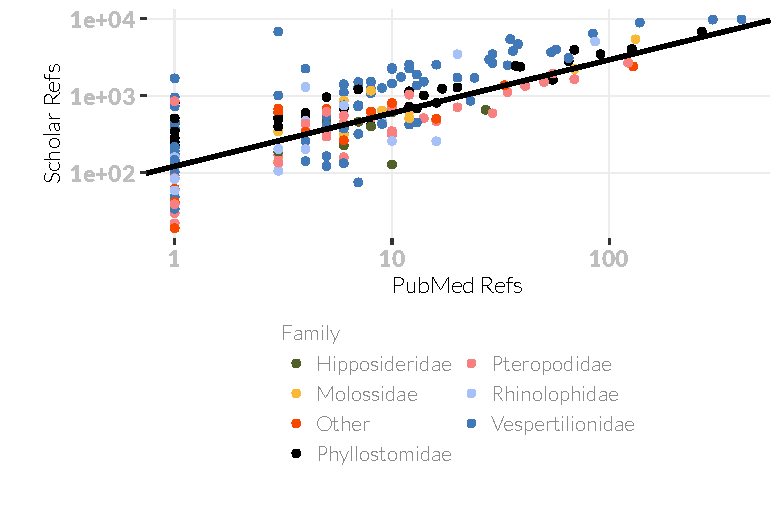
\includegraphics[width=\textwidth]{figure/A-scholarvspubmedPlot-1} 

}

\caption[
  Logged number of references on Scholar and PubMed, with a fitted phylogenetic linear model]{
  Logged number of references on Scholar and PubMed, with a fitted phylogenetic linear model. 
  Colours indicate family. 
  (pgls: $t$ = 19.32, df = 194, $p < 10^{-5}$.)}\label{fig:scholarvspubmedPlot}
\end{figure}


\end{knitrout}















%%-------------------------------------------------------------------------------%%
%% Read full model selection results for both analyses and make tables.
%%-------------------------------------------------------------------------------%%













% latex table generated in R 3.2.4 by xtable 1.8-2 package
% Sun Apr 17 12:14:42 2016
\begin{table}[ht]
\centering
\caption[
  Full model selection results for number of subspecies analysis. 
]{
  Model selection results for number of subspecies analysis. 
  $\bar{\text{AICc}}$ is the mean AICc score across 
inline{nBoots} resamplings of the null random variable. 
  $\Delta$AICc is the model's $\bar{\text{AICc}}$ score minus $\text{min}(\bar{\text{AICc}})$. 
  $w$ is the Akaike weight and can be interpreted as the probability that the model is the best model (of those in the plausible set).
  $\sum w$ is the cumulative sum of the Akaike weights.
  log(Scholar)*NSubspecies implies the interaction term between study effort and number of subspecies.
  } 
\label{A-modelWeights}
\begingroup\tiny
\begin{tabular}{@{}lrrrr@{}}
  \toprule
Model & $\bar{\text{AICc}}$ & $\Delta$AICc & $w$ & $\sum w$ \\ 
  \midrule
log(Scholar)*NSubspecies + log(Scholar) + NSubspecies + log(Mass) + log(RangeSize) & 882.33 & 0.00 & 0.38 & 0.38 \\ 
  log(Scholar)*NSubspecies + log(Scholar) + NSubspecies + log(Mass) & 883.71 & 1.39 & 0.19 & 0.57 \\ 
  log(Scholar)*NSubspecies + log(Scholar) + NSubspecies + log(Mass) + rand & 884.56 & 2.24 & 0.12 & 0.70 \\ 
  log(Scholar)*NSubspecies + log(Scholar) + NSubspecies & 885.47 & 3.14 & 0.08 & 0.78 \\ 
  log(Scholar)*NSubspecies + log(Scholar) + NSubspecies + log(RangeSize) & 885.51 & 3.18 & 0.08 & 0.86 \\ 
  log(Scholar)*NSubspecies + log(Scholar) + NSubspecies + log(RangeSize) + rand & 886.27 & 3.94 & 0.05 & 0.91 \\ 
  log(Scholar)*NSubspecies + log(Scholar) + NSubspecies + rand & 886.28 & 3.95 & 0.05 & 0.96 \\ 
  log(Scholar) + NSubspecies + log(Mass) + log(RangeSize) & 889.26 & 6.93 & 0.01 & 0.97 \\ 
  log(Scholar) + NSubspecies + log(Mass) + log(RangeSize) + rand & 890.13 & 7.80 & 0.01 & 0.98 \\ 
  log(Scholar) + NSubspecies + log(Mass) & 890.66 & 8.34 & 0.01 & 0.99 \\ 
  log(Scholar) + NSubspecies + log(Mass) + rand & 891.59 & 9.26 & 0.00 & 0.99 \\ 
  log(Scholar) + NSubspecies & 892.30 & 9.98 & 0.00 & 0.99 \\ 
  log(Scholar) + NSubspecies + log(RangeSize) & 892.31 & 9.98 & 0.00 & 1.00 \\ 
  log(Scholar) + NSubspecies + log(RangeSize) + rand & 893.15 & 10.82 & 0.00 & 1.00 \\ 
  log(Scholar) + NSubspecies + rand & 893.19 & 10.86 & 0.00 & 1.00 \\ 
  log(Scholar) + log(Mass) + log(RangeSize) & 897.19 & 14.86 & 0.00 & 1.00 \\ 
  log(Scholar) + log(Mass) + log(RangeSize) + rand & 898.05 & 15.72 & 0.00 & 1.00 \\ 
  log(Scholar) + log(Mass) & 898.36 & 16.03 & 0.00 & 1.00 \\ 
  log(Scholar) + log(RangeSize) & 899.13 & 16.80 & 0.00 & 1.00 \\ 
  log(Scholar) & 899.20 & 16.87 & 0.00 & 1.00 \\ 
  log(Scholar) + log(Mass) + rand & 899.26 & 16.94 & 0.00 & 1.00 \\ 
  log(Scholar) + log(RangeSize) + rand & 899.95 & 17.63 & 0.00 & 1.00 \\ 
  log(Scholar) + rand & 900.06 & 17.73 & 0.00 & 1.00 \\ 
  NSubspecies + log(Mass) + log(RangeSize) + rand & 906.60 & 24.27 & 0.00 & 1.00 \\ 
  NSubspecies + log(Mass) + log(RangeSize) & 907.03 & 24.70 & 0.00 & 1.00 \\ 
  NSubspecies + log(RangeSize) & 914.05 & 31.73 & 0.00 & 1.00 \\ 
  NSubspecies + log(RangeSize) + rand & 914.85 & 32.52 & 0.00 & 1.00 \\ 
  NSubspecies + log(Mass) & 920.11 & 37.79 & 0.00 & 1.00 \\ 
  NSubspecies + log(Mass) + rand & 921.06 & 38.73 & 0.00 & 1.00 \\ 
  NSubspecies & 923.37 & 41.04 & 0.00 & 1.00 \\ 
  NSubspecies + rand & 924.26 & 41.94 & 0.00 & 1.00 \\ 
  log(Mass) + log(RangeSize) & 924.61 & 42.28 & 0.00 & 1.00 \\ 
  log(Mass) + log(RangeSize) + rand & 924.68 & 42.35 & 0.00 & 1.00 \\ 
  log(RangeSize) & 931.53 & 49.20 & 0.00 & 1.00 \\ 
  log(RangeSize) + rand & 932.35 & 50.02 & 0.00 & 1.00 \\ 
  log(Mass) & 941.11 & 58.78 & 0.00 & 1.00 \\ 
  log(Mass) + rand & 942.07 & 59.75 & 0.00 & 1.00 \\ 
  Intercept only & 943.72 & 61.39 & 0.00 & 1.00 \\ 
  rand & 944.64 & 62.31 & 0.00 & 1.00 \\ 
   \bottomrule
\end{tabular}
\endgroup
\end{table}




% latex table generated in R 3.2.4 by xtable 1.8-2 package
% Sun Apr 17 12:14:42 2016
\begin{table}[ht]
\centering
\caption[
  Full model selection results for number of effective gene flow analysis. 
]{
  Model selection results for number of effective gene flow analysis. 
  $\bar{\text{AICc}}$ is the mean AICc score across 
inline{nBoots} resamplings of the null random variable. 
  $\Delta$AICc is the model's $\bar{\text{AICc}}$ score minus $\text{min}(\bar{\text{AICc}})$. 
  $w$ is the Akaike weight and can be interpreted as the probability that the model is the best model (of those in the plausible set).
  $\sum w$ is the cumulative sum of the Akaike weights.
  } 
\label{A-fstModelWeights}
\begingroup\scriptsize
\begin{tabular}{@{}lrrrr@{}}
  \toprule
Model & $\bar{\text{AICc}}$ & $\Delta$AICc & $w$ & $\sum w$ \\ 
  \midrule
log(Scholar) + Gene Flow + log(Mass) & 70.57 & 0.00 & 1.00 & 1.00 \\ 
  log(RangeSize) & 104.66 & 34.09 & 0.00 & 1.00 \\ 
  log(Mass) & 105.62 & 35.06 & 0.00 & 1.00 \\ 
  Gene Flow + log(Mass) & 107.45 & 36.88 & 0.00 & 1.00 \\ 
  rand & 110.97 & 40.40 & 0.00 & 1.00 \\ 
  log(Mass) + rand & 113.96 & 43.40 & 0.00 & 1.00 \\ 
  Gene Flow + log(Mass) + rand & 116.98 & 46.41 & 0.00 & 1.00 \\ 
  Gene Flow + rand & 118.94 & 48.37 & 0.00 & 1.00 \\ 
  log(Scholar) + log(Mass) + rand & 120.29 & 49.72 & 0.00 & 1.00 \\ 
  log(Scholar) + Gene Flow + log(Mass) + rand & 122.68 & 52.11 & 0.00 & 1.00 \\ 
  log(Scholar) + log(Mass) + log(RangeSize) + rand & 124.08 & 53.52 & 0.00 & 1.00 \\ 
  log(Scholar) + rand & 125.67 & 55.10 & 0.00 & 1.00 \\ 
  log(RangeSize) + rand & 126.07 & 55.50 & 0.00 & 1.00 \\ 
  log(Scholar) + log(Mass) & 126.52 & 55.95 & 0.00 & 1.00 \\ 
  log(Scholar) & 126.62 & 56.05 & 0.00 & 1.00 \\ 
  log(Mass) + log(RangeSize) + rand & 127.51 & 56.94 & 0.00 & 1.00 \\ 
  log(Scholar) + log(Mass) + log(RangeSize) & 128.01 & 57.44 & 0.00 & 1.00 \\ 
  log(Scholar) + log(RangeSize) & 128.11 & 57.54 & 0.00 & 1.00 \\ 
  log(Scholar) + log(RangeSize) + rand & 128.94 & 58.38 & 0.00 & 1.00 \\ 
  log(Scholar) + Gene Flow & 129.13 & 58.56 & 0.00 & 1.00 \\ 
  log(Scholar) + Gene Flow + log(Mass) + log(RangeSize) + rand & 129.14 & 58.57 & 0.00 & 1.00 \\ 
  log(Scholar) + Gene Flow + rand & 129.18 & 58.61 & 0.00 & 1.00 \\ 
  Gene Flow + log(RangeSize) + rand & 129.29 & 58.72 & 0.00 & 1.00 \\ 
  log(Mass) + log(RangeSize) & 129.50 & 58.93 & 0.00 & 1.00 \\ 
  log(Scholar) + Gene Flow + log(Mass) + log(RangeSize) & 130.80 & 60.24 & 0.00 & 1.00 \\ 
  log(Scholar) + Gene Flow + log(RangeSize) & 130.92 & 60.35 & 0.00 & 1.00 \\ 
  Gene Flow + log(Mass) + log(RangeSize) + rand & 131.18 & 60.61 & 0.00 & 1.00 \\ 
  Gene Flow + log(Mass) + log(RangeSize) & 131.85 & 61.28 & 0.00 & 1.00 \\ 
  log(Scholar) + Gene Flow + log(RangeSize) + rand & 132.59 & 62.02 & 0.00 & 1.00 \\ 
  Gene Flow + log(RangeSize) & 133.12 & 62.56 & 0.00 & 1.00 \\ 
  Gene Flow & 135.79 & 65.22 & 0.00 & 1.00 \\ 
  Intercept only & 136.23 & 65.66 & 0.00 & 1.00 \\ 
   \bottomrule
\end{tabular}
\endgroup
\end{table}








%%-------------------------------------------------------------------------------%%
%% Read and plot bat clocks rocks tree.
%%-------------------------------------------------------------------------------%%









\begin{knitrout}\footnotesize
\definecolor{shadecolor}{rgb}{0.969, 0.969, 0.969}\color{fgcolor}\begin{figure}[t]

{\centering 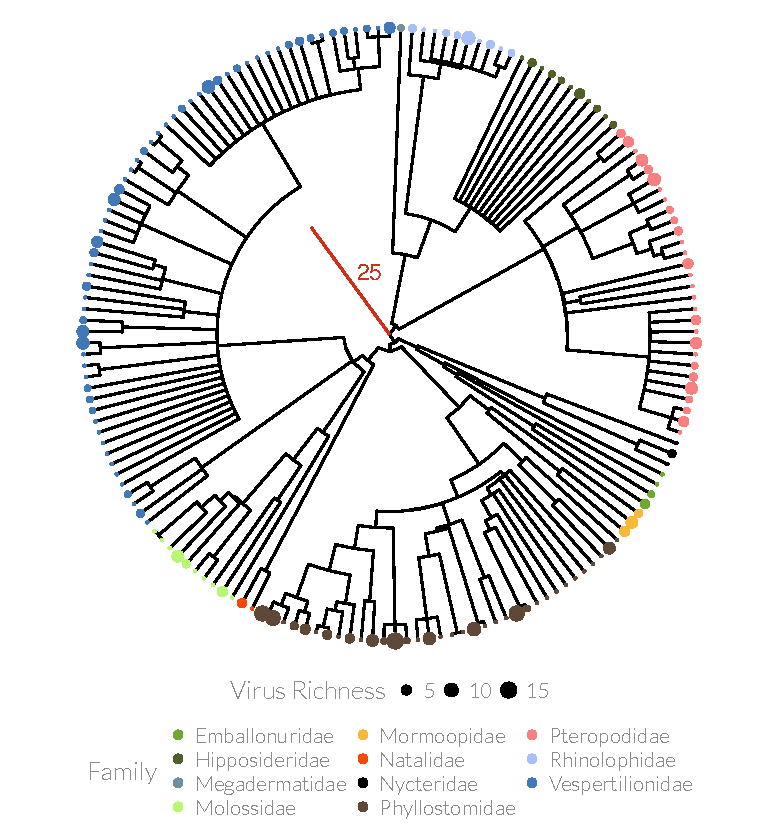
\includegraphics[width=1\textwidth,trim = 0cm 0cm 0cm 0cm]{figure/A-treePlot2-1} 

}

\caption[Pruned alternative phylogeny with dot size showing number of pathogens and colour showing family.]{
Phylogeny from \textcite{jones2005bats} (version 2) pruned to include all species used in the number of subspecies analysis.
Dot size shows the number of known viruses for that species and colour shows family.
Analyses run with this phylogeny gave qualitatively similar results to analyses using the phylogeny from \cite{bininda2007delayed}.
}\label{fig:treePlot2}
\end{figure}


\end{knitrout}






%%-----------------------------------------------------------------------------%%
Interactive plots
%%-----------------------------------------------------------------------------%%







 		






